\documentclass[12pt,a4paper,oneside]{book} % twoside for draf

%\usepackage{babel}
\usepackage[utf8]{vietnam}
\usepackage[english]{babel}
%\usepackage{times}
\usepackage{graphicx}
\usepackage{subcaption}
\usepackage{hyperref}
\usepackage{mathptmx}	% same Time New Roma
%\renewcommand{\rmdefault}{phv} % Arial
%\renewcommand{\sfdefault}{phv} % Arial
\usepackage{url}

%link to part by click on contents region
\usepackage{hyperref}
\hypersetup{
    colorlinks,
    citecolor=black,
    filecolor=black,
    linkcolor=black,
    urlcolor=black
}

\usepackage{fancyhdr}
\usepackage{algorithm2e}
\usepackage{amsmath}
\usepackage{array,tabularx}
\usepackage{amsfonts}
\usepackage{amssymb}
\usepackage{cases}
\usepackage{tabularx}
\usepackage{adjustbox}
\usepackage{multirow}
\usepackage[stable]{footmisc}

\usepackage{bkthesis}

\usepackage{tikz}
\usetikzlibrary{shapes,arrows}

\newenvironment{conditions*}
  {\par\vspace{\abovedisplayskip}\noindent
   \tabularx{\columnwidth}{>{$}l<{$} @{${}:{}$} >{\raggedright\arraybackslash}X}}
  {\endtabularx\par\vspace{\belowdisplayskip}}

\tikzstyle{blank} = [text badly centered, node distance = 2cm, inner sep=0pt]
\tikzstyle{block} = [rectangle, draw, 
    text width=2em, text centered, minimum height=2em]
\tikzstyle{line} = [thick, -latex']
\tikzstyle{startstop} = [rectangle, rounded corners, minimum width=3cm, minimum height=1cm,text centered, draw=black]
\tikzstyle{io} = [trapezium, trapezium left angle=70, trapezium right angle=110, minimum width=3cm, minimum height=1cm, text centered, draw=black]
\newcolumntype{b}{>{\hsize=1.0\hsize}X}
\tikzstyle{process} = [rectangle, minimum width=3cm, minimum height=1cm, text width=7cm ,text centered, draw=black]
\tikzstyle{decision} = [diamond, minimum width=1cm, minimum height=1cm,text width=5cm,aspect=3, text centered, draw=black]
\tikzstyle{arrow} = [thick,->,>=stealth',auto]
\crname{THESIS PROPOSAL}
\ctname{Virtual Assistant using Machine Learning}
\cstuname{
	Student: \\
	\begin{tabular}{ l c }
		Nguyễn Minh Huy & MSSV: 15xxxxx\\
		Nguyễn Lâm Nguyên Bảo & MSSV: 15xxxxx
	\end{tabular}
}

\csCouncil{Computer Science}
\csSupervise{Nguyễn Đức Dũng, Ph.D}
\csReviewer{}
\cttime{11/2021}

\thesislayout

\begin{document}
%-	Bìa cứng - màu xanh dương, chữ mạ vàng (xem mẫu đính kèm)
%-	Trang tên (tờ lót): chất liệu giấy, nội dung giống như bìa LV
%-	Ở gáy LV: in nhan đề LV (có thể in tóm tắt nếu nhan đề quá dài), size 15 – 17
%-	Phiếu Nhiệm vụ LV, chấm điểm Hướng dẫn & Phản biện (đã ký): nhận từ GVHD & GVPB sau khi bảo vệ (theo lịch hẹn).
%-	Lời cam đoan
%-	Lời cảm ơn/ Lời ngỏ
%-	Tóm tắt LV
%-	Mục lục
%-	Danh mục, bảng biểu, hình ảnh, ... (nếu có)
%-	Nội dung LV
%-	Danh mục TL tham khảo
%-	Phụ lục (nếu có)

\coverpage
\frontmatter

% add content here
%-	Lời cam đoan
\begin{declaration}
We assure you that this is our work under the supervision of Nguyễn Đức Dũng, Ph.D. The contents of our research and its results are completely transparent and haven't been released before. The statistics we used during our analysis are either derived from our work or collected from different sources, we also infer other work and results in our content, all of which will be included in the references.
\newline
\indent If any plagiarism was caught in our thesis, we will take full responsibility for our mistakes. Ho Chi Minh City National University, University of technology has no knowledge or connection to the plagiarism that exist in our thesis when we wrote it.
\end{declaration}
~

\begin{acknowledgments}

Acknowledgment.
	
\end{acknowledgments}
~

%
\begin{abstract}
Abstract của báo cáo.
2
\end{abstract}
 

% sử dụng các phần bên dưới nếu cần:
\tableofcontents
%\listofsymbols
%\listoftables
\listoffigures
%\listofalgorithms


\mainmatter

\fancypagestyle{plain}{%
\fancyhf{}
\fancyfoot[LE, RO]{\thepage}
\renewcommand{\headrulewidth}{0.0pt}
}

\pagestyle{fancy}
\renewcommand{\chaptermark}[1]{\markboth{\MakeUppercase{#1}}{}}
\fancyhf{}
\fancyhead[LE,RO]{\leftmark}
\fancyhead[RE,LO]{}
\fancyfoot[LE,RO]{\thepage}
\renewcommand{\footrulewidth}{0.4pt}

%\fancyhead{}  % Clears all page headers and footers
%\rhead{\thepage}  % Sets the right side header to show the page number
%\lhead{}  % Clears the left side page header
%\fancyfoot[positions]{footer}
%\renewcommand{\footrulewidth}{0.4pt}

%\pagestyle{fancy}  % Finally, use the "fancy" page style to implement the FancyHdr headers


\chapter{Introduction}
    
\section{Motivation}

\section{Scope of our topic}
    Our VA application will be composed of four components:
    \begin{itemize}
        \item Trigger word detection (TWD)
        \item Speech recognition (SR)
        \item Natural language understanding (NLU)
        \item Text-to-speech (TTS)
    \end{itemize}
    The purpose of each follows:
    \begin{enumerate}
        \item TWD: The trigger word detection acts a switch to the application. When not in use, the application will be passively listening in the background through the TWD system. When the user says the trigger word, the TWD system will send a signal to other components, activating them and allow the user to engage in conversion with the VA.
        \item SR: When the application is in its active state, voice commands from the user will be transcribed into text through this component. For this project we limit the scope of the SR system to transcribing English only.
        \item NLU: This component interprets the commands from the user using a Machine Learning model trained to detect Intent and Slot-filling. It determines, from the command given, what job to perform and what information has been provided for such job.
        \item TTS: Allows the application to response back to the user verbally, helping to create a completed user experience.
    \end{enumerate}
    
    Each component listed above is in itself a topic that has been researched and studied extensively in the field, from both independent researchers and major corporations such as Google, Apple, etc.In our project we aim to combine the result of studies in the fields into a complete and functional product.
    
    Due to time constraints we can only implement the TWD and NLU component ourselves. The other components(SR and TTS) will be included through the use of open-source codes or public libraries. As mentioned above, the VA is limited to only operate in English, although the TWD will allow the use of any arbitrary  word/phrase as a trigger. The sections below contain the lists of objective we hope to achieve for the application as a whole, as well as individual components.

\subsection{Overall application}
    The ultimate objective of this project is the creation of a convenient, easy-to-use VA application that provides users with the standard of features (i.e. looking up topics, scheduling, unit and currency conversion, etc.) and also allows room for custom commands to fit their needs.
    
    Below is the list of goals we hope to achieve with our application overall:
    \begin{itemize}
        \item Lightweight, low resource consumption
        \item Quick and easy setup
        \item Provide standards features of Voice activation, Voice searching and other Voice commands
        \item Allow custom commands from the user
    \end{itemize}
\subsection{Trigger word detection}
    The trigger word system is the switch that starts the conversation between the user and the VA. Since it needs to constantly listen for the trigger, our first constraint on it will have to be power and resource consumption. Errors in this type of systems often fall into two categories: Not detecting the correct utterances and Detecting incorrect ones. Addressing both would be a tall order, therefore we decided to priority preventing the latter case, seeing how most finds a VA triggering in the middle of an unrelated conversation vastly more infuriating than having to repeat the trigger word an extra 1-2 time(s).  In mathematical terms, we are aiming for decent precision without compromising too much overall recall.
    
    Lastly, the system needs to be able to set up itself quickly with only few recordings from the user as samples. We also aim for the language independence, not restricting the user to any specific wake word/phrase.

    To sum up, out Trigger word system has to achieve to  following:
    \begin{itemize}
        \item Low power and resource consumption
        \item Speaker-dependant detection for personal use
        \item Arbitrary wake word
        \item Quick setup with user recorded samples.
        \item Achieve high precision ( >=80\%) and acceptable recall (>=50\%)
    \end{itemize}
\subsection{NLU}
When designing a virtual assistant, one of the most crucial tasks is to create and train a model for NLU (Natural language understanding) to process the user's input. The first step to accomplish this task is converting speech to text since our users will be communicating with our virtual assistant via speech. However, due to the limitations of our resources, we will not attempt to tackle this problem. Instead, we will be using a python library to convert speech to text (SpeechRecognition) to process the user's command.
\newline
\indent The next step is to create and train a model that can understand the user's commands. Understanding the user's commands means that our model has to accomplish two main jobs. It has to be able to detect the user's intention and extract key information in the user's command to carry out the task. The baseline for our model is that it should be able to understand and carry out tasks that fall under the following list of intentions:
\begin{itemize}
    \item Query: Perform a web search of the topic 
    \item Definition: Read out definition of word/ phrases
    \item News: Read out some news headline
    \item Alarm: set an alarm
    \item Timer: set a timer
    \item Math: perform calculation
    \item Currency exchange
    \item Unit conversion
    \item Calendar: read out events on calendar
    \item Calendar update: Make changes to calendar
    \item Play song: play a song
    \item What song: list out current song
    \item Next song
    \item Weather: get forecast
    \item Date: get current date
    \item Time: get current time
    \item Tell joke
    \item Answer yes/no question
    \item Repeat
    \item Spelling
    \item Random: get random number  
    \item Launch: open program/ website
    \item Hint: list tasks the app can do
\end{itemize}


\chapter{Background knowledge}

    In this chapter we will go over theoretical bases for our project, Section 1 covers the necessary knowledge for Trigger word detection, including the general pipeline, processing of input of audio, the Dynamic Time Warping(DTW) algorithm and MFCC feature extraction.

\section{Knowledge on Trigger word detection}
    \subsection{Trigger word}
    Trigger words, also referred to as Wake words, or Wake-up words, are defined as words or short phrases used to start a conversation with a voice assistant. While in its passive state, a VA constantly listens and waits to detect the preset trigger out of the continuous audio stream. If a detection returns positive, the VA will then switch to its active state, in which it will engage in conversation with the user. 
    
    There are generally two ways of implementing a wake word system, Universal and Personal\cite{snips}. Universal systems are based on Deep Learning models trained on a massive data set of voices. They excels at detecting when anyone say the wake word, but only the set wake words they have been trained for.
    
    Personal systems, on the other hand, operate locally with only a few samples provided by the user. This allows the detection of any arbitrary wake word, at the cost of not working when some other person says the wake word.
    In this project, we decided to use a Personal system for our application, keeping inline with our high customizability design.
    
    \subsection{Wake word detection with Dynamic Time Warping}
    As previously mentioned, personal wake word systems operate with only a few sample utterances from the user. These utterances are stored as templates to be used for template-matching. The matching process is typically done with the Dynamic Time Warping(DTW) algorithm, which measures the similarity of time sequences, including audio. The main idea is to have the application continuously takes audio input that will then be compared with the set of t emplates using DTW. Any resulting similarity score(s) above a certain threshold would indicate a positive utterance has been detected.
    
    The overall pipeline for our system is depicted in this diagram:
    \newline
    \begin{figure}[h]
        \centering
        
        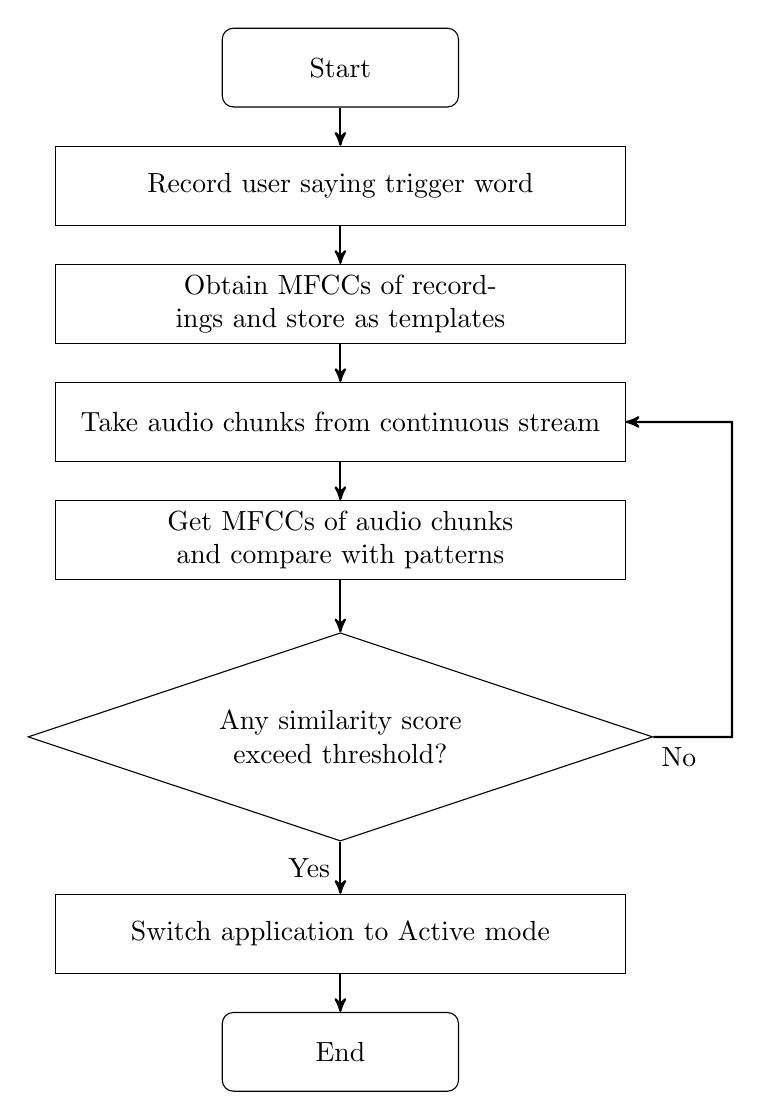
\begin{tikzpicture}[node distance=1.5cm]
        \node (start) [startstop] {Start};
        \node (pro1) [process, below of=start] {Record user saying trigger word};
        \node (pro2) [process, below of= pro1] {Obtain MFCCs of recordings and store as templates};
        \node (pro3) [process, below of = pro2] {Take audio chunks from continuous stream};
        \node (pro4) [process, below of = pro3] {Get MFCCs of audio chunks and compare with patterns};
        \node (dec1) [decision, below of=pro4, yshift = -1cm] {Any similarity score exceed threshold?};
        \node (pro5) [process, below of= dec1,yshift = -1cm] {Switch application to Active mode};
        \node (end) [startstop, below of = pro5] {End}; 
        \draw [arrow] (start) -- (pro1);
        \draw [arrow] (pro1) -- (pro2);
        \draw [arrow] (pro2) -- (pro3);
        \draw [arrow] (pro3) -- (pro4);
        \draw [arrow] (pro4) -- (dec1);
        \draw [arrow] (dec1) -- node[anchor=east] {Yes} (pro5);
        \draw [arrow] (dec1.east) -- ++(1,0) -- ++(0,4) -- node[anchor=north,yshift = -4cm] {No} (pro3.east);
        \draw [arrow] (pro5) -- (end);
        \end{tikzpicture}
        \caption{Trigger word detection flowchart}
        \label{fig:twd}
    \end{figure}
    
    
    We first setup the system be having the user records three utterances of the trigger word, similar to how Google Assistant sets up by requiring the user to say "Okay Google" three times. These three recordings would go to the Pre-processing block to trim out unnecessary details, keeping only relevant audio. Mel Frequency Cepstrum Coefficient (MFCC) Vectors are obtained for each recording and stored as reference templates.
    
    In run time, the wake word engine takes frames from the continuous audio stream, obtain their MFCC vectors and compared those with the stored templates. If a similar match is found, a signal is sent to activate the rest of the application. 
    
    \subsection{Processing audio}
    
    \subsubsection{Template recording}
    The principle of our detection system is to compare incoming audio to a set of templates provided by the user. As such, the first step is to acquire said templates. Since we have no real way of knowing the exact length of the wake word audio, only a margin it will fit into. We  give each utterance up to 3 seconds to record, although in practice utterances rarely surpass 2 seconds of time. The sample rate for our recording is 16000Hz, i.e. 16000 samples is taken per second. Each recording therefore consists of 48000 samples initially.
    
    The next step is noise reduction. We do not expect every users to be in a perfectly quiet environment when recording templates or using the application. Hence, removing background noise is a necessary step to ensure better detection. The noise reduction algorithm we used follows the outline provided by Audacity on their algorithm. \footnote{\url{https://wiki.audacityteam.org/wiki/How_Audacity_Noise_Reduction_Works}} 
    The algorithm first use Fourier Analysis to find the frequency spectrum of the audio. It then find any frequencies whose volume is not louder than the average level and reduce them in volume, keeping the loud vocal wile minimizing smaller background. This is technique is referred to as spectral noise gating. \footnote{\url{https://en.wikipedia.org/wiki/Noise_gate}}
    
    The first pass of noise reduction is done over just noise. For each windowed sample of the sound, we take a Fast Fourier Transform (FFT) using a Hann window and then statistics, including the mean power, are tabulated for each frequency band.

    During the noise reduction phase, those statistics and the Sensitivity setting determine a threshold for each frequency band. We start by setting a gain control for each frequency band such that if the sound has exceeded the threshold, the gain is set to 0 dB, otherwise the gain is set lower to the Noise Reduction slider setting (e.g. -18 dB), to suppress the noise.

    Then time-smoothing is applied (so that the gain for each frequency band moves slowly), followed by frequency-smoothing (so that a single frequency is never suppressed or boosted in isolation).
    
    The output of noise reduction is illustrated below:
    
    \begin{figure}[h]
        \centering
        \begin{subfigure}{0.9\textwidth}
        \includegraphics[width = \linewidth]{img/Figure_1.png}
        \caption{Before}
        \label{fig:noise1}
        \end{subfigure}
        
        \begin{subfigure}{0.9\textwidth}
        \includegraphics[width = \linewidth]{img/Figure_2.png}
        \caption{After}
        \label{fig:noise2}
        \end{subfigure}
    \caption{Noise reduction}
    \label{fig:noise}
    \end{figure}
    
    After noise reduction, we trim the result audio, as silence portions preceding and following the utterance itself are not useful. Once again following the article from Snips \cite{snips}, our trimming process consists of three stages:
    \begin{itemize}
        \item Dividing the signal into small chunks (framing)
        \item Computing the energy of each frame
        \item Removing every frame which energy is lower than a predefined threshold.
    \end{itemize}
    The energy of a frame is the mean of the squares of the signal. A classic approach is to compute the energy of each frame, and compare it to a predefined threshold to classify the frame as silence or not. To increase robustness, a threshold on the ratio of energies between the energy of each frame, and the energy of the frame with highest energy. If this ratio is below 20 decibels, the frame is classified as silence. Below is an example of a trimmed signal:
    
    \begin{figure}[h]
        \centering
        \includegraphics[width = 0.9\textwidth]{img/Figure_3.png}
        \caption{Trimmed signal}
        \label{fig:trimmed}
    \end{figure}
    
    After trimming, the recordings are ready to be converted into template patterns by transforming them into MFCCs, the process of which is covered below, and stored away. 
    
    \subsubsection{Continuous audio stream}
    The Trigger word detection system needs to constantly listen in the background for utterances of the trigger word. As such its input comes in the form of a continuous audio stream. We need a way to extract portions of this stream to compare with our pattern. This is handled by applying a basic sliding window over the stream. An important detail is the size of the window itself. The window should be as close to the length  of the templates as possible, as a high difference in length can vastly affect the similarity obtained from DTW (see below). To counteract this, we dynamically adjust the window size by the average length of the templates. 

    \begin{figure}[h]
        \centering
        \includegraphics{img/window.png}
        \caption{Sliding window over continuous stream\footnote{\url{https://stackoverflow.com/questions/55874826/feature-extraction-for-keyword-spotting-on-long-form-audio-using-a-cnn}}}
        \label{fig:window}
    \end{figure}

    \subsection{Dynamic Time Warping algorithm}
    Dynamic Time Warping is an effective algorithm for measuring time-series similarity which minimizes the effects of shifting and distortion in time by allowing "elastic" transformation of time series in order to detect similar shapes with different phases \cite{DTW}. The algorithm has seen extensive use in speech recognition \cite{sakoechiba}. Two sequences $X = (x_1, x_2, ... , x_A), A \in N $ and $Y = (y_1, y_2, ... , y_B), B \in N $ representing time-series or feature vectors are compared in $O(AB)$ time to yield a metric $d$ representing their similarity. This value is referred to as  the distance or cost of the sequences. Intuitively $d$ will be small for similar sequences and large for different ones. This value is calculated through finding the optimal alignment path (or warping path) representing the most effective way to "warp" X into Y, by mapping elements in X to elements in Y. To do this we construct a Distance matrix $C \in R^AxB$ containing all pairwise distances in X and Y. Each element $C_{i,j}$ corresponds to the distance between $x_i$ and $y_j$.   The warping path $W = w_1, w_2, ... , w_K $ defines this mapping, with $w_k = (x_i,y_j)_k, max(A,B) <= K <= A+B+1$ 
    $W$ follows the following constrains \cite{chu2002iterative}:
    \begin{itemize}
        \item Boundary condition: $w_1 = (1,1)$and $w_k = (A,B)$. The warping path must start and end in diagonally opposite corners of the cost matrix.
        \item Continuity: Given $w_k = (a,b)$ then $w_{k-1} = (a',b')$, where $a - a'<= 1$ and $b - b'<= 1$. This restricts the allowable steps in the warping path to adjacent cells (including diagonally adjacent cells)
        \item Monotonicity: Given $w_k = (a,b)$ then $w_{k-1} = (a',b')$, where $a - a' >= 0$ and $b - b' >= 0.$ This forces the points in $W$ to be monotonically spaced in time, as indices can only stay the same or increase. 
    \end{itemize}
    There are many paths that satisfy these constrains, but we are only interested in the path with lowest cost 
    \begin{equation}
        DTW(A,B) = min(\sum_{k=1}^K w_k)        
    \end{equation}
    The generation of $C$ is defined as follows:
    \begin{equation}
         C_{i,1} = \sum_{k=1}^i dist(x_i,y_1), i \in [1,A] 
    \end{equation}
     \begin{equation}
        C_{1,j} = \sum_{k=1}^j dist(x_1,y_k)  , j \in [1,B]
    \end{equation}
    \begin{equation}
        C_{i,j} = dist(x_i , y_j) + min(C_{i-1,j} , C_{i,j-1} , C_{i-1,j-1} ) , i \in [2,A] , j \in [2,B] 
    \end{equation}
    Once the cost matrix is built, the optimal path follows the path with minimum cost from (A,B) back to (1,1). This path, illustrated in the figure below, can be used as a presentation on the similarity of the sequences. The closer it is to the main diagonal line, the more similar the sequences are. Additionally, path constrains\cite{DTW} such as slope and window constrains can be applied to limit the warping path, preventing it from straying too far from the diagonal line. These can help avoid unnecessary comparisons for obviously different sequences, but may also miss out on correct utterances. The distance or similarity $d$ is the cumulative sum of distances between respective points of the signal, and can be interpreted from the last element of the cost matrix C[A,B]. However, as $d$ is calculated as a cumulative sum, it is somewhat proportional to the length of the sequences i,e, two nearly similar long sequences may give the same distance as two different, but shorter sequences. Therefore, an extra step is needed to make this result universal (independent of the wake word), done by normalizing it by the length of the warping path.
    
    
    \begin{figure}[h]
        \centering
        \includegraphics[width = 0.9\textwidth]{img/The-optimal-warping-path-aligning-time-series-from-the-Figure-1.jpg}
        \caption{The optimal warping path aligning two time series\cite{DTW}}
        \label{figdtwpath}
    \end{figure}
    
    \subsection{Mel-Frequency Cepstrum Coefficients for DTW}
    While the DTW algorithm can be applied for two raw audio sequences, in practice it is almost never viable to do so. Considering two clips of audio 1 second long sampled at 16000Hz would be represented as two sequences of dimensions (16000,1). Applying DTW will require the construction of a (16000,16000) cost matrix at $O(16000^2)$ time. As such, most uses feature extractions techniques, which captures the overall representation of an audio sequence in a much smaller set of features. One of the most popular among them is the Mel-Frequency Cepstrum Coefficients, due to how it approximates how a human ear would perceive audio more closely than other techniques. MFCC has two
    types of filter which are spaced linearly at low frequency
    below 1000 Hz and logarithmic spacing above 1000Hz. A
    subjective pitch is present on Mel Frequency Scale to capture important characteristic of phonetic in speech.\cite{muda}  
    The overall process of MFCC feature extraction follows:
    \newpage
    \begin{figure}
        \centering
        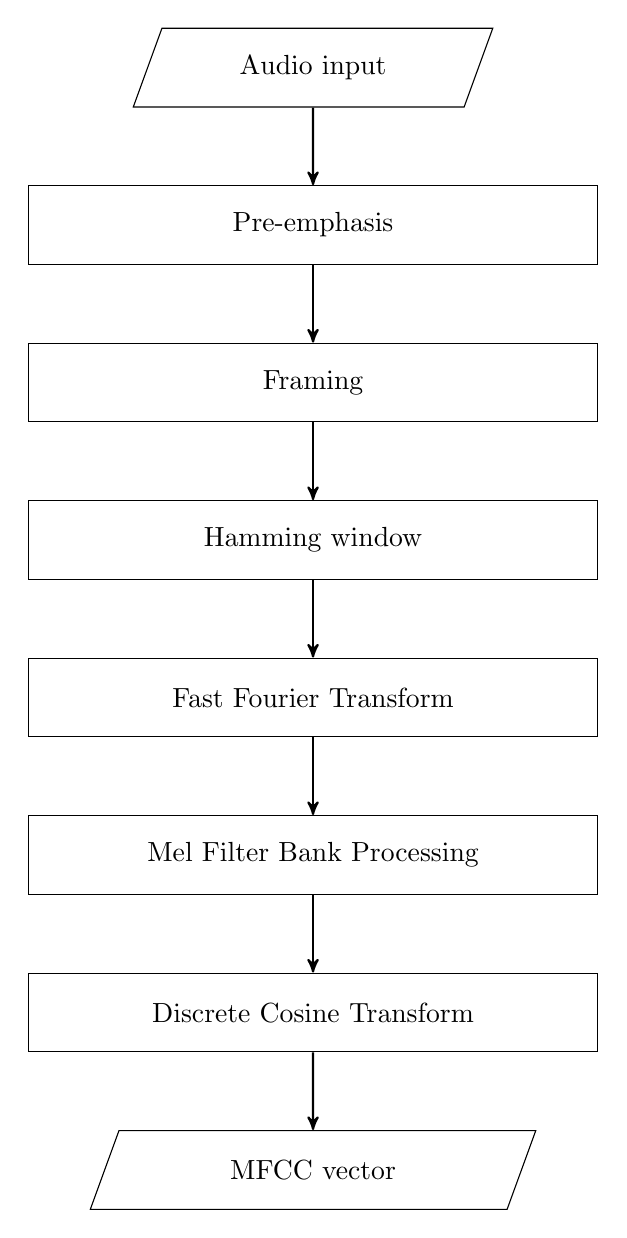
\begin{tikzpicture} [node distance=2cm]
        \node (inp) [io]  {Audio input};
        \node (pro1) [process, below of = inp] {Pre-emphasis};
        \node (pro2) [process, below of = pro1] {Framing};
        \node (pro3) [process, below of = pro2] {Hamming window};
        \node (pro4) [process, below of = pro3] {Fast Fourier Transform};
        \node (pro5) [process, below of = pro4] {Mel Filter Bank Processing};
        \node (pro6) [process, below of = pro5] {Discrete Cosine Transform};
        \node (out) [io, below of = pro6] {MFCC vector};  
        \draw [arrow] (inp) -- (pro1);
        \draw [arrow] (pro1) -- (pro2);
        \draw [arrow] (pro2) -- (pro3);
        \draw [arrow] (pro3) -- (pro4);
        \draw [arrow] (pro4) -- (pro5);
        \draw [arrow] (pro5) -- (pro6);
        \draw [arrow] (pro6) -- (out);
        \end{tikzpicture}
        \caption{MFCC process}
        \label{fig:mfcc_flow}
    \end{figure}
    Step 1: Pre-emphasis.
    This optional step puts the signal through a high frequency filter which increases the power for signals at higher frequencies. This balances out the signal and improve the overall signal-to-noise ratio. The coefficient $a$ used typically ranges from 0.90 to 0.99.
    \begin{equation}
        Y(n) = X(n) -aX(n-1)
    \end{equation}
    
    Step 2: Framing. 
    This step separates the audio input into fixed-sized frames ranging from 20ms to 40ms in length, with a typical overlap from 10ms to 20ms between two adjacent frames. Each frame would contain N samples, typically 256 or 512.
    
    Step 3: Hamming window.
    A Hamming window is a windowing function that integrates all the closest frequency lines together, minimizing the signal discontinuities at the start and end of each frame.It achieves this effect by shrinking the values of the signal at the start and end of the frame toward zero. The equation for Hamming window is given as:
    \begin{itemize}
        \item W(n): Hamming Window function, $0<=n<=N - 1$
        \item N: number of sample each frames
        \item Y(n): Output signal
        \item X(n): Input signal
        
    \end{itemize}
    \begin{equation}
        Y(n) = X(n) * W(n)
    \end{equation}
    \begin{equation}
        W(n) = 0.54 - 0.46 cos(\frac{2n\pi}{N-1}), 0 <=n <= N-1 
    \end{equation}
    
    Step 4: : Fast Fourier Transform.
    The Fourier Transform algorithm is applied to convert N samples from each frame from time domain into frequency domain. The basis of Fourier Transform was implemented in 2000 by Alexander and Sakidu. \cite{ftbasis} There, its purpose is to convert the convolution of the glottal pulse $U[n]$ and the vocal tract impulse response $H[n]$ in the time domain. This statement supports the equation below:
    \begin{equation}
        Y(w) = FFT[h(t)*x(t)] = H(w) x X(w)
    \end{equation}
    If $X(w)$, $H(w)$ and $Y(w)$ are the Fourier Transform of $X(t)$, $H(t)$ and $Y(t)$ respectively. Fast Fourier Transform is used as an optimized algorithm for calculating the above transformation.
    
    Step 5 : Mel Filter Bank Processing.
    The frequencies obtained from the previous step will then be mapped into the Mel scale using triangular filters:
    \begin{figure}[h]
        \centering
        \includegraphics[width=0.9\textwidth]{img/Mel-scale-filter-bank-from-young-et-al-1997-6.png}
        \caption{Mel scale filter bank, from (young et al,1997)\cite{sharma}}
        \label{fig:melscale_filter}
    \end{figure}
    
    The triangle filters are used to compute a weighted sum of filter spectral components so that the output fits into a Mel scale. Each filter’s magnitude frequency response is triangular in shape and equal to unity at the centre frequency and decrease linearly to zero at centre frequency of two adjacent filters. The output of each filter is the sum of its filtered spectral components. After that the following equation is used to compute the Mel scale value for given frequency f in HZ:  
    \begin{equation}
        F(Mel Scale) = [2595 *log_{10}(1+f)700]
    \end{equation}
    
    Step 6: Discrete Cosine Transform
    This step the log Mel spectrum above back into time domain using Discrete Cosine Transform (DCT). The result obtained is the Mel Frequency Cepstrum Coefficients. At this stage, MFCCs are ready to be formed into feature vectors for use in DTW. The input signal now has the form of a $NxM$ matrix, with $N$ as the number of frames and $M$ as the number of coefficients. A visualization of the input signal and output matrix is presented below:
    \begin{figure}
        \centering
        \begin{subfigure}{0.9\textwidth}
        \includegraphics [width = \linewidth]{img/Figure_3.png}
        \caption{Input signal}
        \label{fig:mfcc1}
        \end{subfigure}
        \begin{subfigure}{0.9\textwidth}
        \includegraphics[width = \linewidth]{img/mfcc.png}
        \caption{Output MFCC}
        \label{fig:mfcc2}
        \end{subfigure}
        \caption{MFCC result}
        \label{fig:mfcc}
    \end{figure}
    
\newpage    
    
\section{Knowledge on NLU}
\subsection[title]{Speech-to-Text basics\footnote{\url{https://cloud.google.com/speech-to-text/docs/basics#synchronous-recognition}}}
\subsubsection{Speech-to-Text API recognition} 
The simplest way to perform recognition on speech audio data is to use a Speech-to-Text API synchronous recognition request. Speech-to-Text can process a speech audio data with length up to 1 minute sent in a synchronous request. After that, Speech-to-Text processes and recognizes all of the word in the audio file and return a response.
\newline
\indent A synchronous request is blocking, meaning that Speech-to-Text must return a response before processing the next request. Speech-to-Text typically processes audio faster than real-time, processing 30 seconds of audio in 15 seconds on average. In cases of poor audio quality, your recognition request can take significantly longer.
\subsubsection{Synchronous Speech Recognition Requests}
All Speech-to-Text API synchronous recognition requests must include a speech recognition config field (of type RecognitionConfig). A \path{RecognitionConfig} contains the following sub-fields:
\begin{itemize}
    \item \path{encoding} (required): specifies the format to encode the input audio. A lossless encoding such as \path{FLAC} or \path{LINEAR16} is more preferable for best performence. This sub-field is optional for \path{FLAC} and \path{WAV} file since the encoding has already been included in the file header.
    \item \path{sampleRateHertz} (required): specifies the sample rate (in Hertz) of the input audio. This sub-field is optional for \path{FLAC} and \path{WAV} file since the encoding has already been included in the file header.
    \item \path{languageCode} (required): contains the language + region/locale to use for speech recognition of the input audio. The language code must be a BCP-47 \cite{BCP47} identifier. 
    \item \path{maxAlternatives} (optional, defaults to 1): designates the number of alternative transcriptions to produce in the response. By default, the Speech-to-Text API provides one primary transcription. 
    \item \path{profanityFilter} (optional): indicates whether to filter out profane(offensive) words or phrases. The filtered words or phrases will consist of their first letter and asterisks for the remaining characters (e.g. f***). Note that the profanity filter only works on single word or phrase, it won't be able to detect abusive or offensive speech that is a combination of words.
    \item \path{speechContext} (optional): contain the context of the input audio.
\end{itemize}
\indent Audio is supplied to Speech-to-Text through the audio parameter of type RecognitionAudio. The \path{audio} field contains either of the following sub-fields:
\begin{itemize}
    \item \path{content}: contains the audio pass in to evaluate, embedded within the request. The audio passed within this field is limmited to 1 minute in duration due to the limitation of synchronous recognition.
    \item \path{url}: contains a URI pointing to the audio content. The file must not be compressed.
\end{itemize}
\subsubsection{Speech-to-Text API responses}
As indicated previously, a synchronous Speech-to-Text API response may take some time to return results, proportional to the length of the supplied audio. The respond that the API return will have the following field:
\begin{itemize}
    \item \path{results}: contain the list of results where each result corresponds to a segment of audio. Each will consist of one or more of the \path{alternatives} fields. An \path{alternatives} contains a list of possible transcriptions. The number of alternatives appear depend on whether you requested more than one alternative (by setting \path{maxAlternative} to a specific value) or the Speech-to-Text API can produces an alternative with high enough quality. Each alternative will consist of the following fields: \begin{itemize}
        \item \path{transcript}: contains the transcribed text produced from the input audio.
        \item \path{confidence}: contains a value between 0 and 1 indicating how confident Speech-to-Text is of the given transcription.
    \end{itemize}
\end{itemize}

\subsection{Word Embedding}


\subsection{Intent Detection}

\subsection{Slot filling}

\chapter{Literature surveys}
As stated, this project involves the combination of multiple components, each of which has an extensive research scene behind them. A thorough understanding of  these components, obtained through reviewing research literature, is crucial for implementing them into our project correctly. 

\section{Wake-Up-Word Spotting for Mobile Systems\cite{wuwmobile}}
Our trigger word detection follows the method described in this paper . The paper proposes a system to spot wake-up words in continuous audio for use on a mobile system. The key constraints listed are:  speaker dependent spotting, use of individual personalized keyword, no transcription of the keyword, no training phase, low power and computing resources, and in general a language-independent system. The system is implemented using template-matching  with DTW. Other algorithms such as Euclidian Distance and Cross Correlation are used alongside DTW to increase accuracy.

The aim of the research is to achieve a precision of more than 95\% at an acceptable recall of more than 50\%. This means that about half of the WUW are detected correctly while almost all triggered detection are correct. As the goal is to prioritize precision over recall, motivated by the need to  not triggering too many false alarms, the best combination of the distance measures is determined by weighting the precision three times more important than the recall. Testing in different environments with low, medium and high level of noise yields an average precision of 99.7\% and recall of 56.9\%.
\begin{figure}[h]
    \centering
    \includegraphics[width = 0.9\textwidth]{img/WUW-spotting-system.png}
    \caption{WUW spotting system}
    \label{fig:lr1l}
\end{figure}
\section{Keyword Spotting based on the Analysis of Template Matching Distances\cite{barakat}}
This literature covers a Keyword Spotting(KWS) system to spot certain keywords in continuous speech using spoken example templates. The approach proposed also use DTW for pattern matching, requiring no modelling or training. This article briefly pointed out some limitations of DTW based matching with fixed threshold, alongside other methods for KWS such as Hidden Markov Model (HMM) and phone/word recognizer. When operating with a fixed threshold, DTW models typically suffer problems regarding the computational complexity, determining the appropriate similarity threshold\cite{wilpon} and the poor modeling of word duration.\cite{yadong}

To address this problem, the article introduced the use of the DTW distance histogram for automatic estimation of similarity thresholds for every keyword-utterance pair.This proposed approach depends on a hypothesis that the distance between the word template and sections of the utterance containing the word is small compared with the distance resulting from comparisons of the template with other parts of the utterance that do not contain the word. This should apply regardless of speakers and dialects.The proposed KWS is designed based on this hypothesis; the template is compared with varying length segments,centered at each analysis frame of the utterance, and the resulting minimum distance and corresponding frame number are recorded. 

The entire process is described through the figure included. The result from experiments on various keywords varies, with some giving very high or low recall/precision. The system can achieve a recall higher than 73\% but with low precision. The top two most reasonable setup resulted in 57.5\%, 55\% recall and 44.8\%, 47.6\% precision respectively.
\begin{figure}[h]
    \centering
    \includegraphics[height=15cm]{img/kws_lr2.png}
    \caption{The proposed KWS system}
    \label{fig:lr2}
\end{figure}

\input{chapters/Chapter4.tex}
\input{chapters/Chapter5.tex}
\input{chapters/Chapter6.tex}

\bibliography{refs}{}
\bibliographystyle{plainurl}


%\bibliography{refs}
%\bibliographystyle{plain}
%-	Danh mục TL tham khảo
%-	Phụ lục (nếu có)

\end{document}
